%!TEX root = ..\..\main.tex

\section{Methode}
Lineare Kameramodell wie das projektive Transformation bilden den Weltpunkt, Bildhauptpunkt und das Projektionszentrum auf dem selben optischen Strahl ab. Im idealen Fall werden nach der Transformation alle Bildgeraden wieder als Geraden dargestellt. In der Realität bilden gerade Kamerasysteme mit Weitwinkelobjektiven die Geraden gebogen ab, da die Brennweite klein ist und der Blickwinkel sehr groß~\cite{HartleyRadDist}. Ein weiterer Grund ist ein mangelhaftes Linsendesign mit einer fehlerhaften Krümmung der einzelnen Linsenelementen in einem Objektiv~\cite{WengRadDist}\cite{Zhang:1996:EGT:844381.845228}. Diese verzerrten Abbildungen werden in der Regel als kissenförmig beschrieben und Radiale Linsenverzerrung genannt. In einigen Fällen kann es aber auch zu tonnenförmigen Verzerrungen kommen. Neben den linearen Kamermodellen muss also für die vollständige Nachbildung einer realen Kamera auch die Linsenverzerrung berücksichtigt werden. 

In den nächsten Abschnitten wird im Detail auf die RDF~\cite{HartleyRadDist} und der Levenberg-Marquard-Approximation (LMA)~\cite{LevMarquardt} eingegangen. Die RDF beschreibt das Verhalten der Linsenverzerrung und mit Hilfe der LMA können die entsprechenden Verzerrungskoeffizienten aus korrespondierenden Punktepaaren  approximiert werden. Diese Paare beinhalten stets einen Punkt in der Welt und den entsprechenden Bildpunkt auf den er abgebildet wird.

\subsection{Radial Distance Function (RDF)}
\todo[inline, color=red]{Vera}
Die oben beschriebene kissenförmige Linsenverzerrung ist demzufolge konvex und strikt symmetrisch um die optische Achse~\cite{WengRadDist}. Es kann daher voraus gesetzt werden, dass der Bildhauptpunkt $x_0$ im Zentrum der radialen Verzerrung liegt. In diesem Fall kann die Linsenverzerrung, wie in Formel~\ref{equ:BasicModel} moduliert werden. Hier werden die unverzerrten und linearen Bildkoordinaten als $x_u$ und die verzerrten Bildpunkte als $x_d$ bezeichnet. $L(r)$ definiert die Linsenfunktion des Systems und ist abhängig vom Abstand $r$.

\begin{equation}
\label{equ:BasicModel}
\begin{pmatrix}
x_d \\
y_d\\
\end{pmatrix} =
L(r)
\begin{pmatrix}
x_u-x_0\\
y_u -y_0\\
\end{pmatrix}
\end{equation}

Der Abstand $r$ ist definiert als euklidischer Abstand vom Zentrum $x_0$, wie in Formel~\ref{equ:Abstand} aufgeführt. Aus nummerischen Gründen wird für die Approximation die Form $r^2$ verwendet, welche den Rundungsfehler und den Rechenaufwand minimiert. 

\begin{equation}
\label{equ:Abstand}
r = \sqrt{x_u^2+y_u^2}
\end{equation}

 Für die Linsenfunktion gilt $L(x_0)=1$, da der Betrag der Verzerrung mit zunehmenden Abstand größer wird. $L(r)$ ist für alle weiteren Bildpunkte unbekannt. Daher wird $L(r)$ um $r=0$ mit einer Taylorreihe approximiert (vgl. Formel~\ref{equ:Taylor}). 
 
 \begin{equation}
 \label{equ:Taylor}
 L(r)=1+\kappa_1*r+\kappa_2*r^2+\kappa_3*r^4 + \dots
 \end{equation}

Mit den Koeffizienten $\kappa_1, \kappa_2, \kappa_3, \dots$ kann die radiale Verzerrung des Bildes korrigiert werden und ausgehend von einer quadratischen Approximation gibt sich anhand Formel~\ref{equ:Taylor} die RDF für $x_u$ und $y_u$ mit Formel~\ref{equ:RDF}~\cite{WangRaddist}.

\begin{equation}
\label{equ:RDF}
\begin{split}
x_u = x_d*(1+\kappa_1*r+\kappa_2*r^2+\kappa_3*r^4 + \dots) + x_0\\
y_d = y_d*(1+\kappa_1*r+\kappa_2*r^2+\kappa_3*r^4 + \dots) + y_0
\end{split}
\end{equation}

Die unbekannten Koeffizienten $\kappa_1, \kappa_2, \kappa_3, \dots$ können mit einer nicht-linearen Ausgleichsrechnung approximiert werden indem das Minimierungsproblem mit der RDF moduliert wird. Ein effizientes Verfahren zur Approximierung der Koeffizienten ist die bekannte LMA~\cite{LevMarquardt}.

\subsection{Levenberg-Marquard-Approximation}
\todo[inline, color=red]{Vera}
Die \textit{Methode der kleinsten Quadrate} von Gauß ist ein bekanntes Verfahren, welches die unbekannten Parameter $\alpha$ von überbestimmten Systemen aus linearen oder nichtlinearen Gleichungen annähert. Diese Systeme werden in der Regel aus Wertepaaren moduliert, welche in voraus gemessen und bestimmt wurden. Der Messwert wird im folgenden als $y$ und der als ideale angenommene Wert $t$ bezeichnet.
Im Fall der einer Radialen Entzerrung sollte für die Anzahl der Wertepaare $M>3$ sein um eine gute Näherung der Parameter beziehungsweise Koeffizienten zu ermitteln.
Es handelt sich somit um ein überbestimmtes System, welches nicht exakt lösbar ist. In diesem Fall kann nur verlangt werden, dass die Abweichungen und Residuen minimal sind~\cite{schwarz2011numerische}. 

Für die \textit{Methode der kleinsten Quadrate} wird die euklidische Norm des Residuums $b-Ax$ minimiert~\cite{dahmen2008numerik} und das entsprechende lineare Ausgleichsproblem wird wie in Formel~\ref{equ:LinAusgleich} formuliert. Hier gibt $N$ die Anzahl der Parameter und $M$ die Anzahl der gemessenen Wertepaare an. Die Matrix $A$ enthält die gesuchten Parameter $a_{i,j=1}$ und der Vektor $b$ alle gemessenen Werte.
\begin{equation}
\label{equ:LinAusgleich}
\begin{split}
||Ax^*-b||_2 = \min_{x\in \mathbb{R}^N} ||Ax-b||_2\\
mit\ A\in \mathbb{R}^{M\times N}\ und\ b\in \mathbb{R}^{N}
\end{split}
\end{equation}

Lineare Ausgleichsprobleme können mit einer Vielzahl an verschieden Verfahren gelöst werden, wie zum Beispiel einer \textit{Cholesky}- beziehungsweise QR-Zerlegung oder der Singulärwertzerlegung.
Doch diese Verfahren können nur dann angewendet werden, wenn der Messwert $y$ von allen Parametern linear abhängig ist. Ist dies nicht gegeben, handelt es nicht um ein nichtlineares Ausgleichsproblem, wie bei der RDF (vgl. Formel~\ref{equ:RDF}). Zur Lösung dieser Art von Ausgleichsverfahren werden in der Praxis das \textit{Gauß-Newton-Verfahren} (GMV) und die LMA angwendet. Letzteres ist eine effizientere Weiterentwicklung des GMV und eine geeignete Wahl um die Koeffizienten $\kappa$ der RDF zu approximieren.

Im Sinne der \textit{Methode der kleinsten Quadrate} lässt sich das nichtlineare Ausgleichsproblem wie in Formel definieren~\cite{schwarz2011numerische}. $F(x)$ ist definiert als Abbildung $F: \mathbb{R}^N \arrowvert \mathbb{R}^M$ und $F_i()x:= y(t_i,x)-b_i\ mit\ i= 1,\dots,M$. 

\begin{equation}
\label{equ:LinAusgleich}
\begin{split}
||F(x^*)||_2 = \min_{x\in \mathbb{R}^N} ||F(x)||_2\\
oder\\
\phi(x^*)=\min_{x\in \mathbb{R}^N} ||\phi(x)||_2 = \frac{1}{2}||F(x)||_2^2 = \frac{1}{2}F(x)^TF(x)
\end{split}
\end{equation}
 

\section{System}

\subsection{Ausgleich der radialen Linsenverzerrung}
\todo[inline, color=red]{Vera}

\subsection{Ermittlung der Punktepaare}
\todo[inline, color=yellow]{Artjom}

UnwarpJ erzeugt in der Landmarks-Datei die Punkte-Paare nicht in der Reihenfolge in der die Punkte  gesetzt wurden, deswegen war es nicht möglich die Ziel-Koordinaten zur Laufzeit zu berechnen. Hierzu war es notwendig zuerst in das Ausgangsbild das optimale Gitter einzuzeichnen und danach die Punkt-Paare mit Hilfe von UnwarpJ zu setzen.

Dafür wurden in der Plugin-Klasse die Gitterparameter als Konstanten angelegt und das Zeichnen der Gitterpunkte in der Methode $compute\_draw\_optimal\_Grid()$ realisiert.
%kapitelverweis?

%formeln zur berechnung
Zur Berechnung der Ziel-Koordinaten wurden folgende Werte siehe Tab. \ref{tab:gitter_koordinaten_variablen} genutzt:

\begin{table}[H]
\centering
\begin{tabular}{|l|l|p{0.5\textwidth}|}
\toprule
Variablen-Name & Wert & Funktion\\
\midrule
distCross & 111 & Abstand der Gitter-Kreuzpunkte\\
\midrule
nXCross2Corner & 10 & Anzahl der Gitter-Kreuzpunkte vom Mittelpunkt bis zum Ende des Gitters\\
nYCross2Corner & 6 & \\
\midrule
nCol & 21 & Anzahl der Gitter-Spalten\\
nRow & 13 & Anzahl der Gitter-Reihen\\
\midrule
XgridCenter & 1084 & Gitter-Mittelpunkt \\
YgridCenter & 714 & \\
\bottomrule
\end{tabular}
\caption{Variablen zur Berechnung des optimalen Gitters ausgeführt als Klassenkonstanten}
\label{tab:gitter_koordinaten_variablen}
\end{table}

Zuerst erfolgt die Berechnung des oberen-linken Gittereckpunktes als $x_{offset}$ und $y_{offset}$. 

\begin{equation}
\label{equ:gitter_offset}
\begin{split}
x_{offset} = XgridCenter - nXCross2Corner * distCross\\		 y_{offset} = YgridCenter - nYCross2Corner * distCross
\end{split}
\end{equation}

Danach erfolgt die Berechnung der Kreuzpunkte über eine geschachtelte Schleife für jede Gittter-Reihe und Gitter-Spalte. 

\begin{equation}
\label{equ:gitter_kreuzpunkte}
\begin{split}
x_{undist} = colid * distCross+ x_{offset}\\
y_{undist} = rowid * distCross + y_{offset}
\end{split}
\end{equation}

An diesen Koordinaten müssen nur noch Ovale gezeichnet werden und es entsteht das in Abb. \ref{fig:gitter-optimal} dargestellte Bild, welches nun in UnwarpJ genutzt werden kann.

\begin{figure}[H]
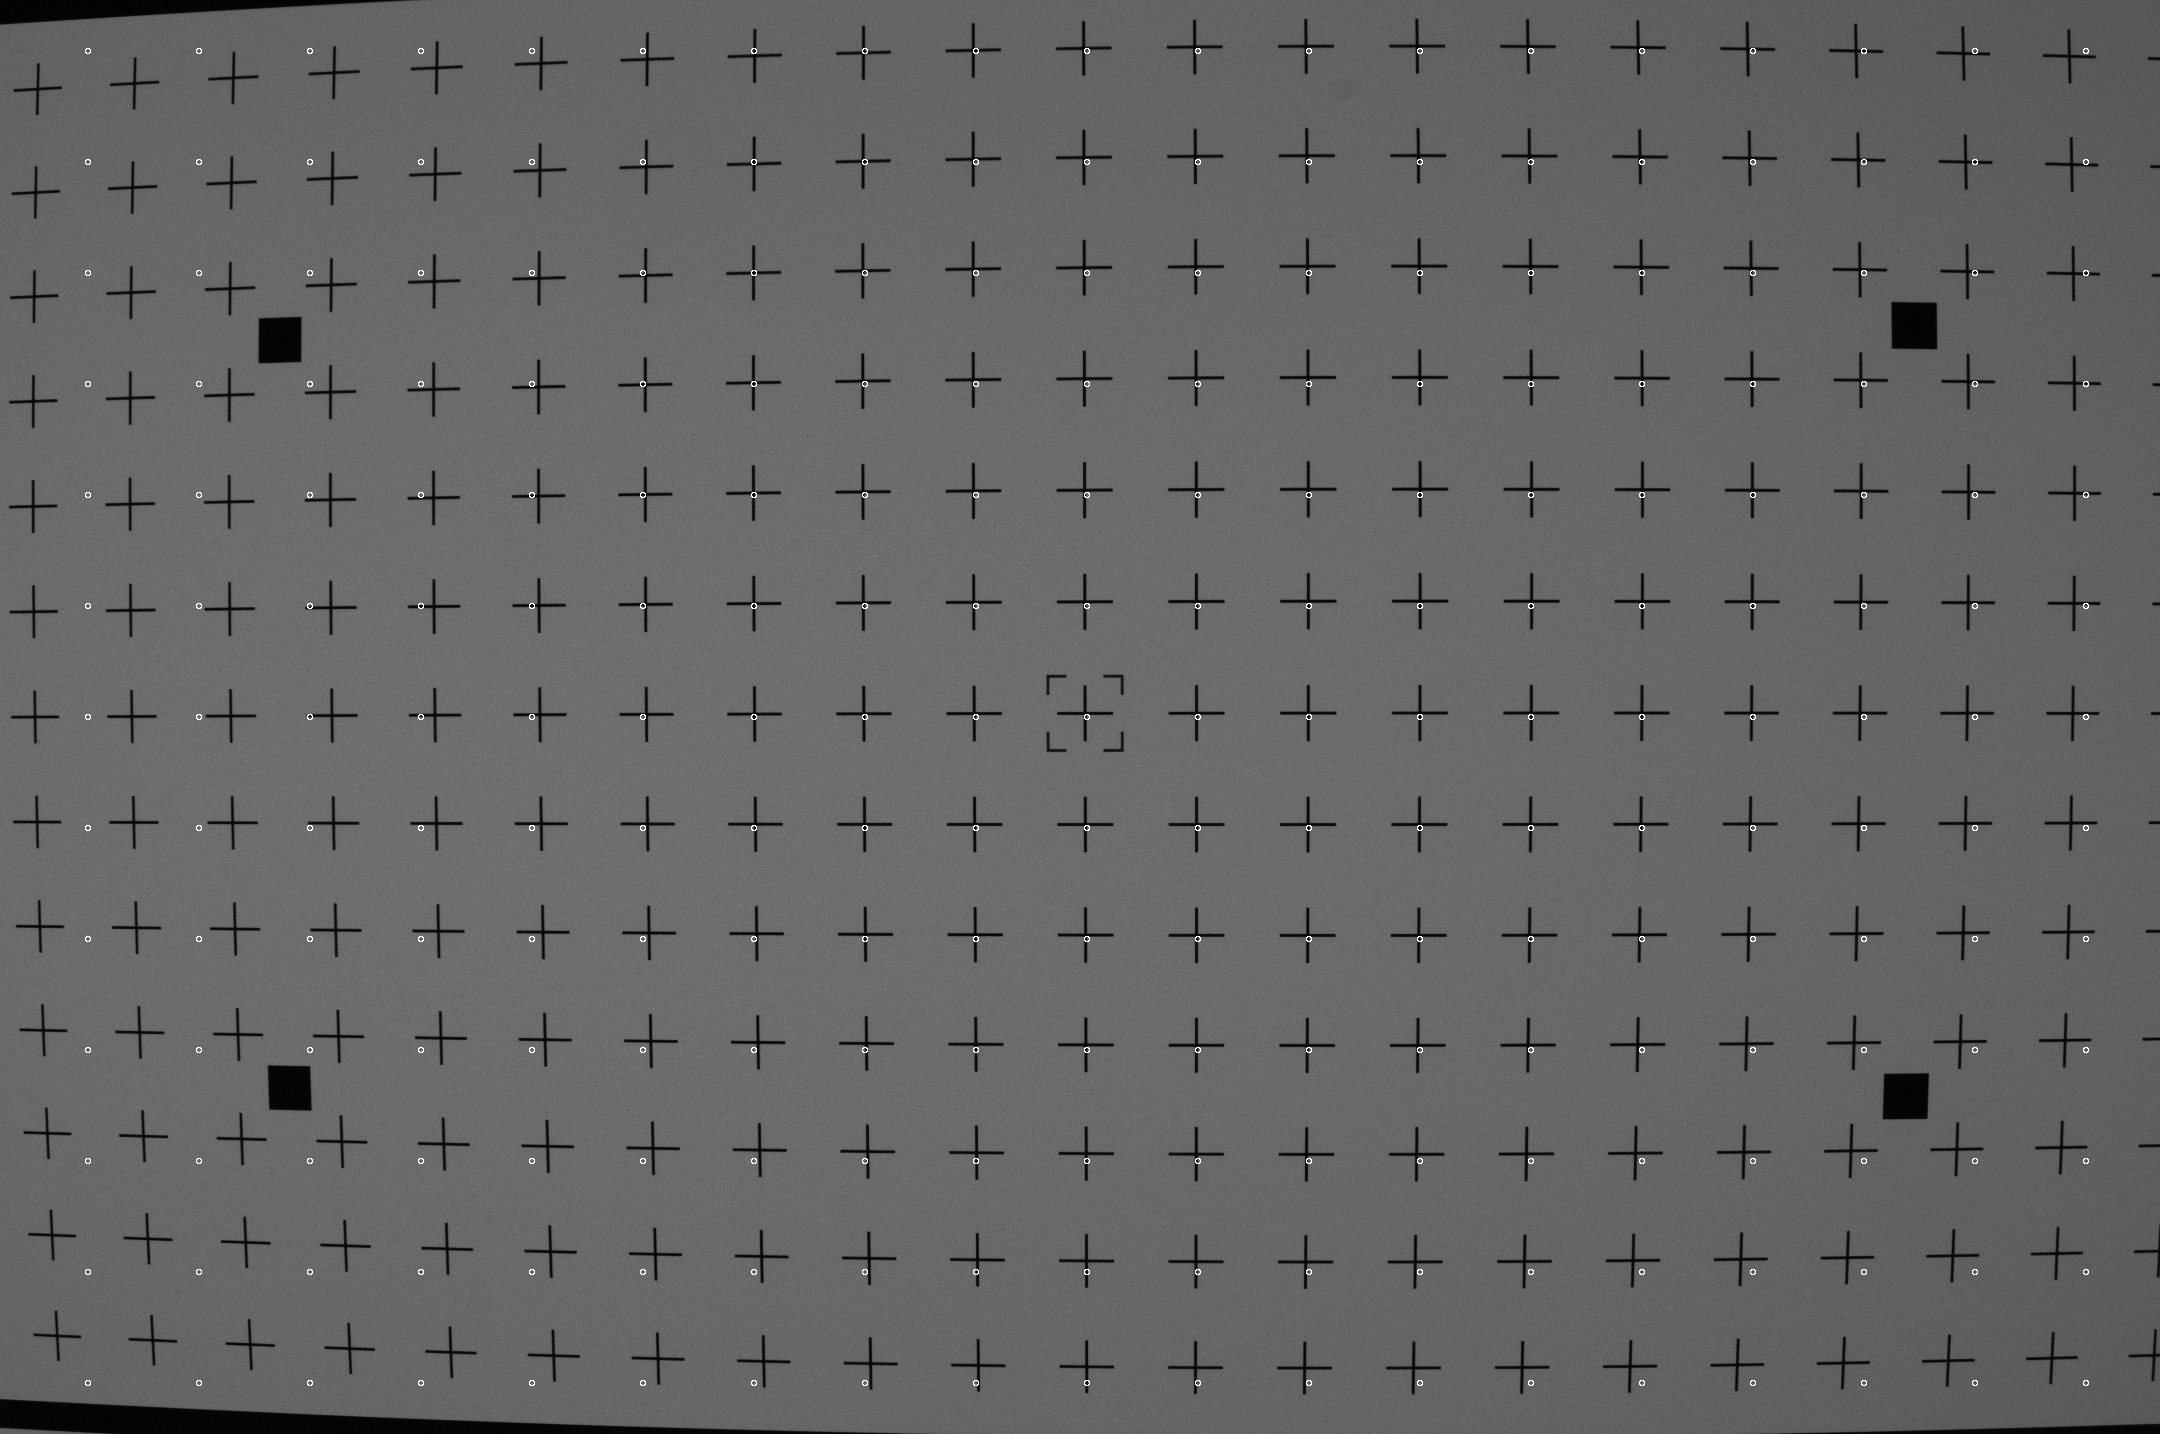
\includegraphics[width=\textwidth]{Images/optimales-gitter.png}
\label{fig:gitter-optimal}
\caption{Erzeugte Zielpunkte mit Hilfe der $compute\_draw\_optimal\_Grid()$ Methode}
\end{figure}

\subsection{Aufstellung des Problems}

\subsection{Initialisierung des Minimierungsproblems}

\subsection{Plugin-Klassen}
\todo[inline, color=yellow]{Artjom}

Im folgenden werden die Methoden der einzelnen Klassen erläutert. Die vollständige UML zur besseren Verständlichkeit der Klassenbeziehungen ist der Abb. \ref{img:UML} zu entnehmen.

\begin{figure}[H]
	\center
	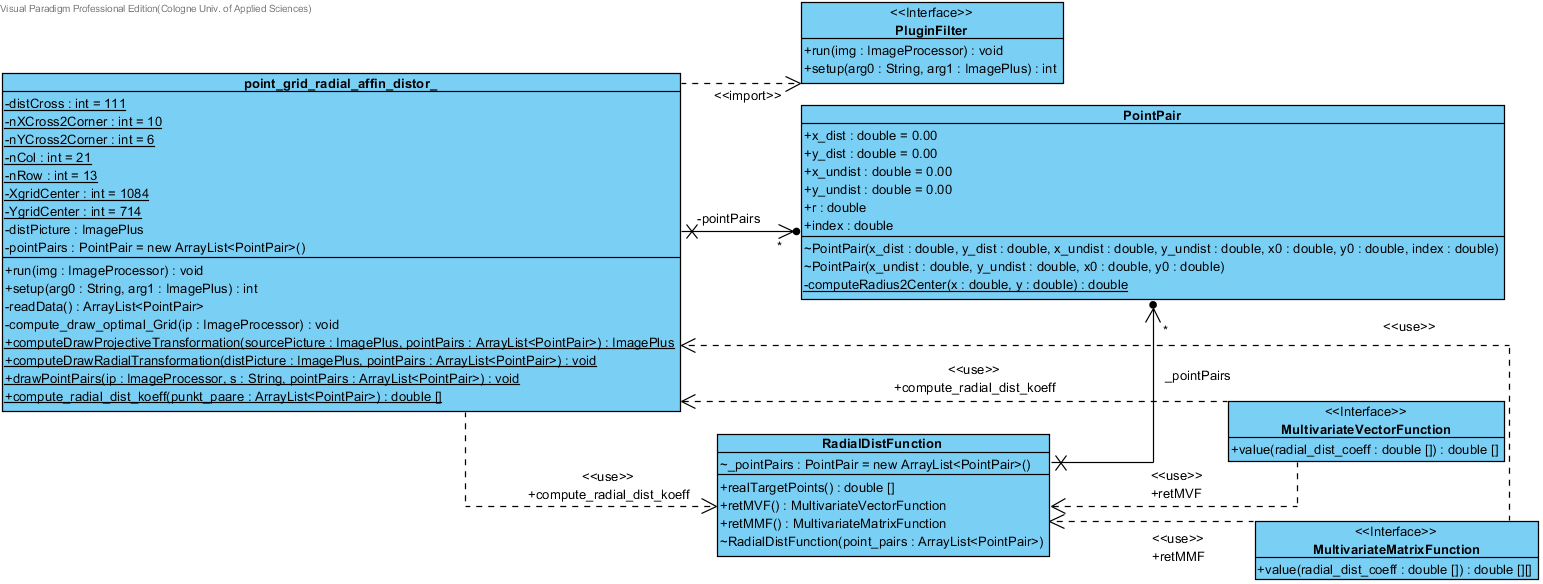
\includegraphics[width=\textheight, angle =90]{Images/Class Diagram1.png}
	\caption{UML Klassendiagramm}
	\label{img:UML}
\end{figure}

\subsubsection{point\_grid\_radial\_affin\_distor\_}
Hauptklasse der Anwendung. Implementiert das Interface \emph{PluginFilter} um über ImageJ aufgerufen werden zu können.

Die Klasse besitzt folgende Methoden und deren Funktion:

\begin{table}[H]
	\begin{tabular}{|p{0.45\textwidth} | p{0.55\textwidth}|} 
		\hline
		run & Main-Methode des PlugIns in der die Optimierung aufgerufen wird\\ \hline
		setup & Konstruktor-Methode des PlugIns mit der die Bildreferenz abgespeichert wird\\ \hline
		compute\_draw\_optimal\_Grid & Berechnung und Abbildung des optimalen Gitters anhand der Klassenkonstanten \\ \hline
		readData & Liest aus einer in ImageJ geöffneten UnwarpJ-Landmarks Datei Punkt-Paare ein für die Start- und Ziel-Koordinaten\\\hline
		computeDrawRadialTransformation & Startet die Berechnung der radialen Verzerrung und zeichnet das dazugehörige entzerrte Bild\\ \hline
		computeDrawProjective-Transformation & Berechnet anhand von Punkpaaren die projektive Transformation und gibt die Abbildung zurück. Zusätzlich werden die Punkt-Paare mit transformiert.\\ \hline
		drawTargets & Zeichnet Punkte an den übergebenen Start- und Ziel-Koordinaten in das übergebene Bild\\ \hline
		compute\_radial\_dist\_koeff & Berechnet mit dem LevenbergMarquadt Optimierer die Koeffizienten der Radialen Verzerrung der übergebenen Punkt und gibt die Koeffizienten zurück\\ 
		\hline
	\end{tabular}
	\caption{Methoden der point\_grid\_radial\_affin\_distor\_ Klasse}
\end{table}

\subsubsection{PointPair}
Eine einfache Klasse zum Speichern der Vorgabe- und Ziel- Koordinaten und des Abstandes zum Mittelpunkt. Sie besitzt einen Konstruktor bei dem der Mittelpunktabstand anhand der Parameter automatisch berechnet und gespeichert wird. Dies ist nützlich, da so der Radius nicht in einem externen Aufruf berechnet werden muss.

\subsubsection{RadialDistFunction}
Klasse zum Erzeugen der Funktionen für den Levenber-Marquadt-Optimierer.

\begin{table}[H]
	\begin{tabular}{|p{0.45\textwidth} | p{0.55\textwidth}|} 
		\hline
		RadialDistFunction & Konstruktor der Klasse. Es wird ein PointPair Array erwartet welcher Koordinaten-Paare für Start- und Ziel-Koordinaten enthält.\\ \hline
		realTargetPoints & Gibt ein Array aus welches nur die Ziel-Koordinaten enthält. Dieses wird für den Optimierer benötigt.\\ \hline
		retMVF & Funktion zur Modellierung der Radialen Verzerrung für den Optimierer. Berechnet zu den Vorgegeben Koeffizienten und einer Start-Koordinate die Ziel-Koordinate\\ \hline
		retMMF & Jacobi-Matrix-Funktion zur Berechnung der Ableitung nach den einzelnen vom Optimierer vorgegebenen Koeffizienten \\ 
		\hline
	\end{tabular}
	\caption{Methoden der RadialDistFunction Klasse}
\end{table}

